\documentclass[a4paper,USenglish]{article}
\usepackage[utf8]{inputenc}
\usepackage[T1]{fontenc,url}
\usepackage{babel,textcomp}
\usepackage{graphicx}
\usepackage[backend=biber,style=numeric-comp]{biblatex}
\usepackage{listings-golang} %% Support Go in listings.
\usepackage{color}
\urlstyle{sf}

\addbibresource{references.bib}
\bibliography{references}

\definecolor{bluekeywords}{rgb}{0.13,0.13,1}
\definecolor{greencomments}{rgb}{0,0.5,0}
\definecolor{redstrings}{rgb}{0.9,0,0}

\lstdefinestyle{goprograms}{
	basicstyle=\footnotesize,
	language=Golang,
	frame=shadowbox,
	numbers=left,
	captionpos=b, % sets the caption-position to bottom.
	numberstyle=\tiny,
	showspaces=false,
	showtabs=false,
	breaklines=true,
	showstringspaces=false,
	breakatwhitespace=true,
	escapeinside={(*@}{@*)},
	commentstyle=\color{greencomments},
	keywordstyle=\color{bluekeywords},
	stringstyle=\color{redstrings},
	basicstyle=\ttfamily
}

\title{Go Abstract Syntax Tree Visualizer}
\author{Christian Bergum Bergersen\\ chrisbbe@ifi.uio.no}

\begin{document}
\maketitle


\begin{abstract}
This article documents a simple tool developed in Go to draw the abstract syntax tree for
Go programs. The abstract syntax tree is drawn with Grapvizer for simplizity.
\end{abstract}

\section{Implementation}
To keep track of the nodes in the tree, the program uses a stack to \texttt{Pop} and \texttt{Push}
nodes on the stack, \texttt{Push} happens each time the program dives a level deeper in the
tree, \texttt{Pop} happens when the program has to go up one level, this way we can track the
relationships between a parent and child node. The \texttt{stack} implementation is taken from
chapter \textbf{1.5 Stack-Custom Types with Methods} in \cite{summerfield:go}.

\section{How to use and results}
Even small programs has a pretty big abstrac syntax tree, which makes it increansingly harder
to visualize all nodes of the abstract syntax tree as the code grows, its best illustrated with
an visualization of the abstract syntax three for the standard \texttt{HelloWorld.go} program as
listed under.

\lstinputlisting[style=goprograms,caption={HelloWorld in Go},label=code:HelloWorld]{../testPrograms/HelloWorld.go}

\begin{figure}[htp]
  \centering
  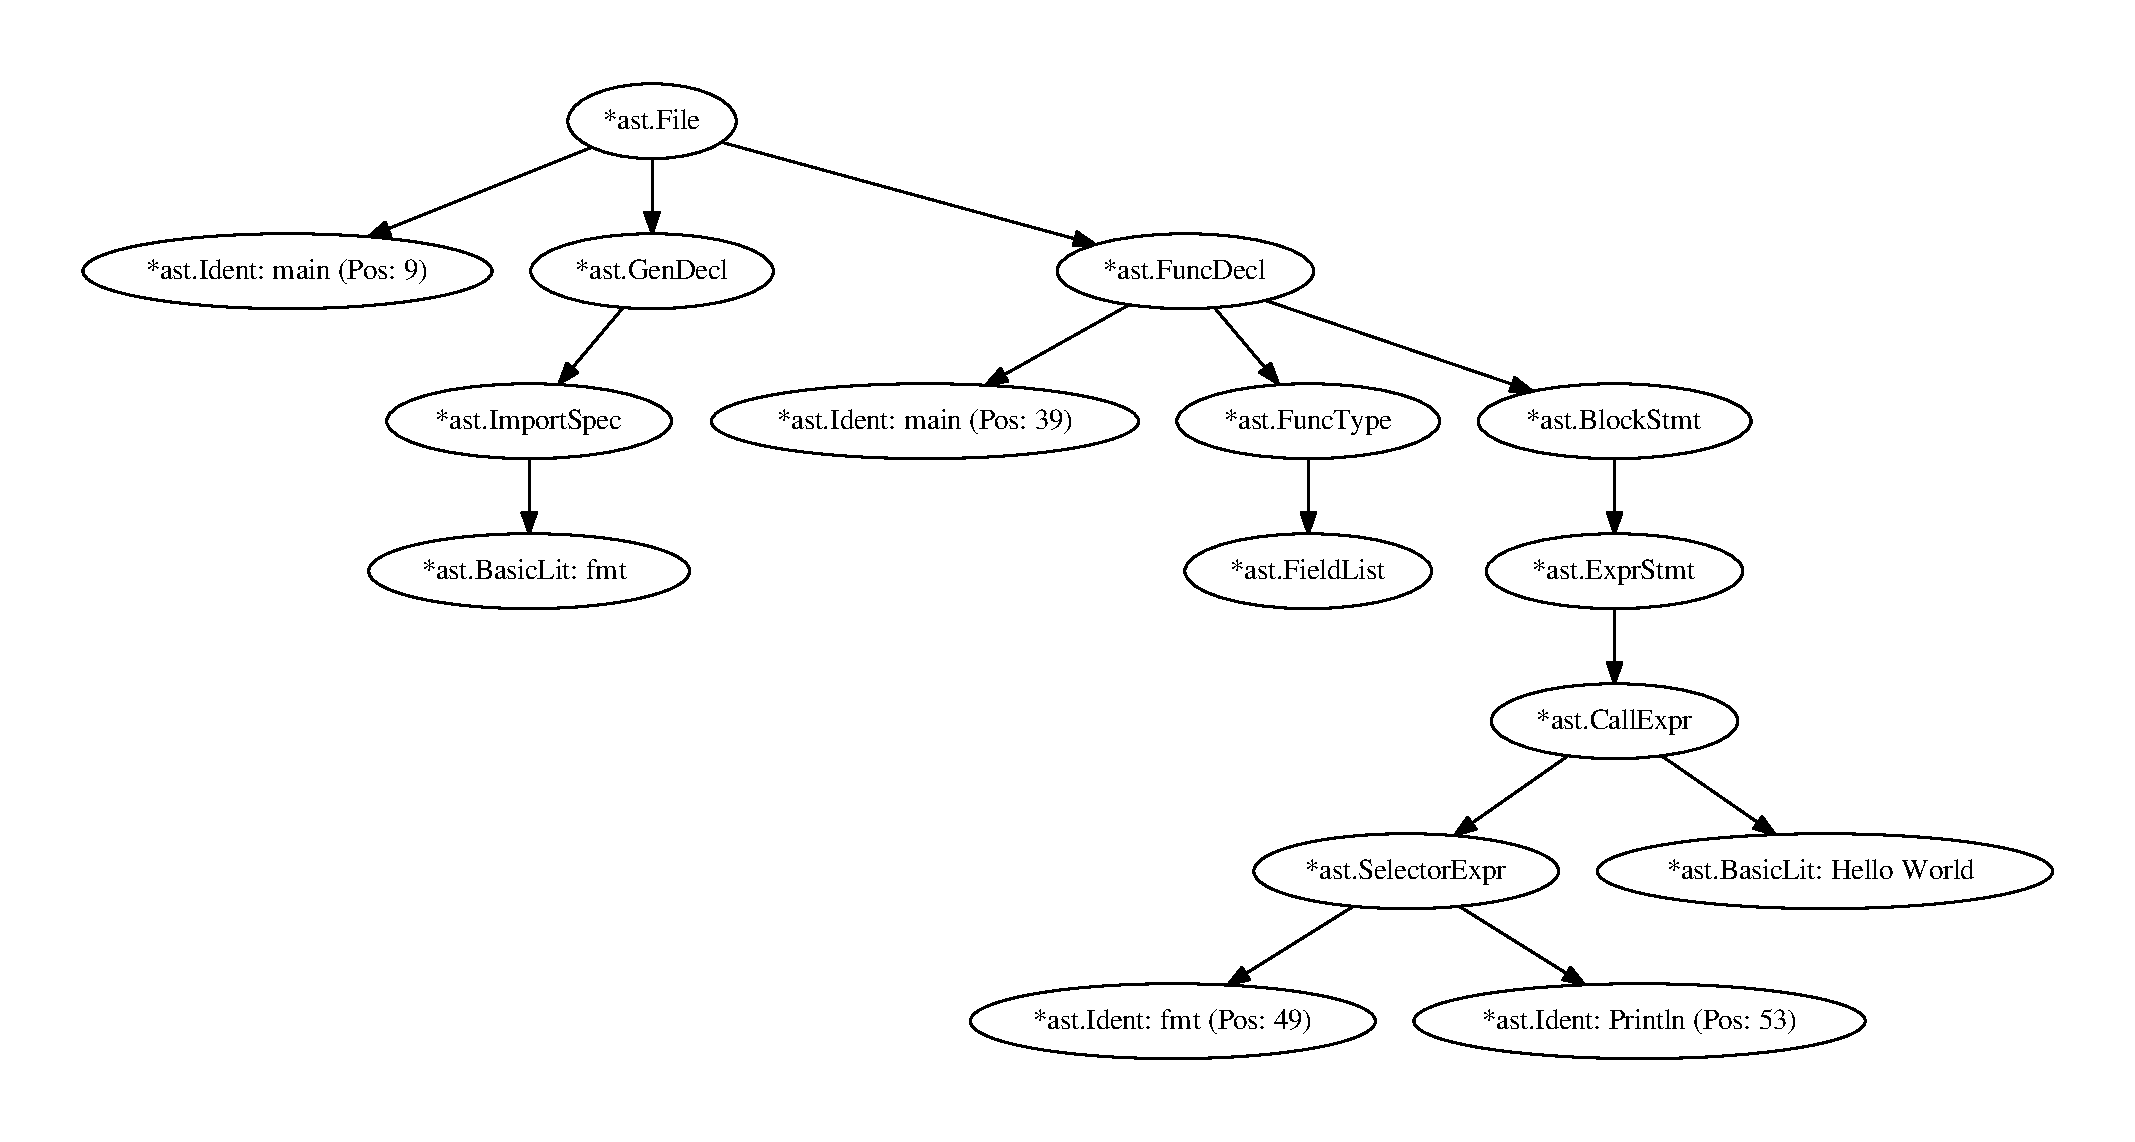
\includegraphics[scale=0.5]{HelloWorld.pdf}
  \label{}
  \caption{Abstract Syntax Tree visualized for the small "HelloWorld.go" Go program.}
\end{figure}

\section{Known problems}
The following list contains known problems and potential improvments for the code.

\begin{enumerate}
	\item The generating of Dotty code doe's not know if there already exist a relationship between
	two nodes, resulting in some situations the graph to have multiple arrows between two or more nodes,
	which does not have any semantic meaning, but syntactically ugly.
\end{enumerate}

\printbibliography

\end{document}
